% \vspace{-3ex}
\begin{figure}[h]
\centering
% \cfbox{box-gray}{
\resizebox{!}{0.17\columnwidth}{
% \tikzsetnextfilename{}
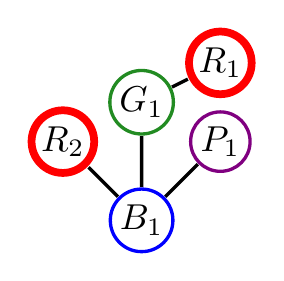
\begin{tikzpicture}[
mynode/.style={draw, circle, very thick, inner sep=1pt, scale=1.3},
myline/.style={draw, very thick},
]
\pgfmathsetmacro{\n}{7};
\pgfmathsetmacro{\r}{1.75};

\node[mynode,draw=red,line width=2.8pt] (1) at (1,0.5) {$\xcolor{R}_1$};
\node[mynode,draw=ForestGreen] (2) at (0,0)  {$\xcolor{G}_1$};
\node[mynode,draw=blue] (3) at (0,-1.5)  {$\xcolor{B}_1$};
\node[mynode,draw=Purple] (4) at (1,-0.5) {$\xcolor{P}_1$};
\node[mynode,draw=red,line width=2.8pt] (5) at (-1,-0.5)  {$\xcolor{R}_2$};

\draw [myline] (1) -- (2);
\draw [myline] (2) -- (3);
\draw [myline] (3) -- (4);
\draw [myline] (3) -- (5);

\end{tikzpicture}
}
\resizebox{!}{0.17\columnwidth}{
\begin{tikzpicture}
\node[] () at (0,-0.5)  {\scalebox{2}{$\Leftrightarrow$}};
\node[] () at (0,0.5)  { };
\node[] () at (0,-1.5)  { };
\end{tikzpicture}
}
% }
% \cfbox{box-gray}{
\resizebox{!}{0.2\columnwidth}{
% \tikzsetnextfilename{}
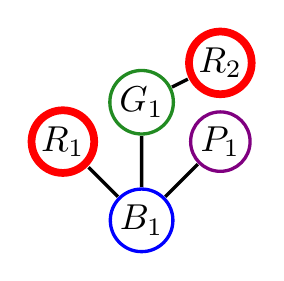
\begin{tikzpicture}[
mynode/.style={draw, circle, very thick, inner sep=1pt, scale=1.3},
myline/.style={draw, very thick},
]
\pgfmathsetmacro{\n}{7};
\pgfmathsetmacro{\r}{1.75};

\node[mynode,draw=red,line width=2.8pt] (1) at (1,0.5) {$\xcolor{R}_2$};
\node[mynode,draw=ForestGreen] (2) at (0,0)  {$\xcolor{G}_1$};
\node[mynode,draw=blue] (3) at (0,-1.5)  {$\xcolor{B}_1$};
\node[mynode,draw=Purple] (4) at (1,-0.5) {$\xcolor{P}_1$};
\node[mynode,draw=red,line width=2.8pt] (5) at (-1,-0.5)  {$\xcolor{R}_1$};

\draw [myline] (1) -- (2);
\draw [myline] (2) -- (3);
\draw [myline] (3) -- (4);
\draw [myline] (3) -- (5);

\end{tikzpicture}
}
% }
\caption{Component-type isomorphism.\label{fig:ch2:ciso}}
\end{figure}
% \vspace{-3ex}